\Chapter{JavaScript implementáció}

\Section{A p5 függvénykönyvtár}

Az elkészült szerkesztő jelentős mértékben támaszkodik a \textit{p5.js} függvénykönyvtár adta lehetőségekre. A következőkben ennek használata kerül röviden bemutatásra.

\SubSection{Használat}

A p5 függvénykönyvtár telepítéséhez csak le kell tölteni azt, majd hozzá kell adni a fájlunkhoz egy \lstinline[style=html]|script| tag segítségével, például:

\begin{lstlisting}[style=html]
<html>
	<head>
		<script src="../p5.min.js"></script>
		<script src="sketch.js"></script>
	</head>
	<body>
	</body>
</html>
\end{lstlisting}

A \textit{p5.js} függvényhívások a \textit{sketch.js}-ben kapnak helyet globális névtér használat esetében:

\begin{lstlisting}[style=es6]
function setup() {
	createCanvas(400, 400);
}

function draw() {
	background(220);
	ellipse(50, 50, 80, 80);
}
\end{lstlisting}

A \textit{setup} függvény a \textit{sketch.js} betöltésekor fut le, célszerű iderakni a p5 vászon létrehozását (\textit{createCanvas} függvényhívás, mely paraméterként várja a magasságot és a szélességet). A \textit{draw} függvény a futás során folyamatosan meghívódik.

A dolgozatban a \textit{p5.js} példányosított módban fut a modulok miatt:

\begin{lstlisting}[style=es6, morekeywords={P5}]


import {setup, draw} from "./canvas/canvas.js";	

const sketch = s => {
	
	s.setup = () => {
		setup();
	}
	
	s.draw = () => {
		draw();
	}

    ...

}

const P5 = new p5(sketch);

export {
	P5
}
\end{lstlisting}

Ebben az esetben a \textit{P5} névtér alá kerül a vászon és a modulokban importálni kell a névtér hivatkozását, valamint az eddig globális \textit{p5.js} függvényhívások is ezen névtér alá kerülnek. A fenti példa így kerül definiálása:

\begin{lstlisting}[style=es6, morekeywords={P5}]
import {P5} from "../sketch.js";

const setup = () => {
	P5.createCanvas(400, 400);
}

const draw = () => {
	P5.background(220);
	P5.ellipse(50, 50, 80, 80);
}
\end{lstlisting}

\Section{Az alkalmazás felépítése}

Az alkalmazás a \ref{fig:block}. ábrán lévő blokkdiagram alapján készült el. Az ábrán lévő elemek nem minden funkcióban jelennek meg. 

A következő fejezetben az egyes funkciók képernyői láthatók. Leírásra kerülnek az adott pont alatt lévő funkciók, és használatuk.

A fejezetben megjelenő képernyő mintaképeken a vászon ötszörös nagyításban van a jobb átláthatóság miatt.

\SubSection{Kezdőképernyő} 

A \ref{fig:canvas}. ábrán látható képernyő jelenik meg az alkalmazás betöltésekor. A bal oldali menüben automatikusan ki van választva a vászon mozgatására alkalmas funkció.

Az egér bal gombjával tudjuk pozicionálni, míg görgővel kicsinyíteni vagy nagyítani a vásznat. Az egér középső gombját lenyomva pedig az alapértelmezett pozícióra és nagyításra visszaáll a vászon.

\begin{figure}[!h]
	\centering
	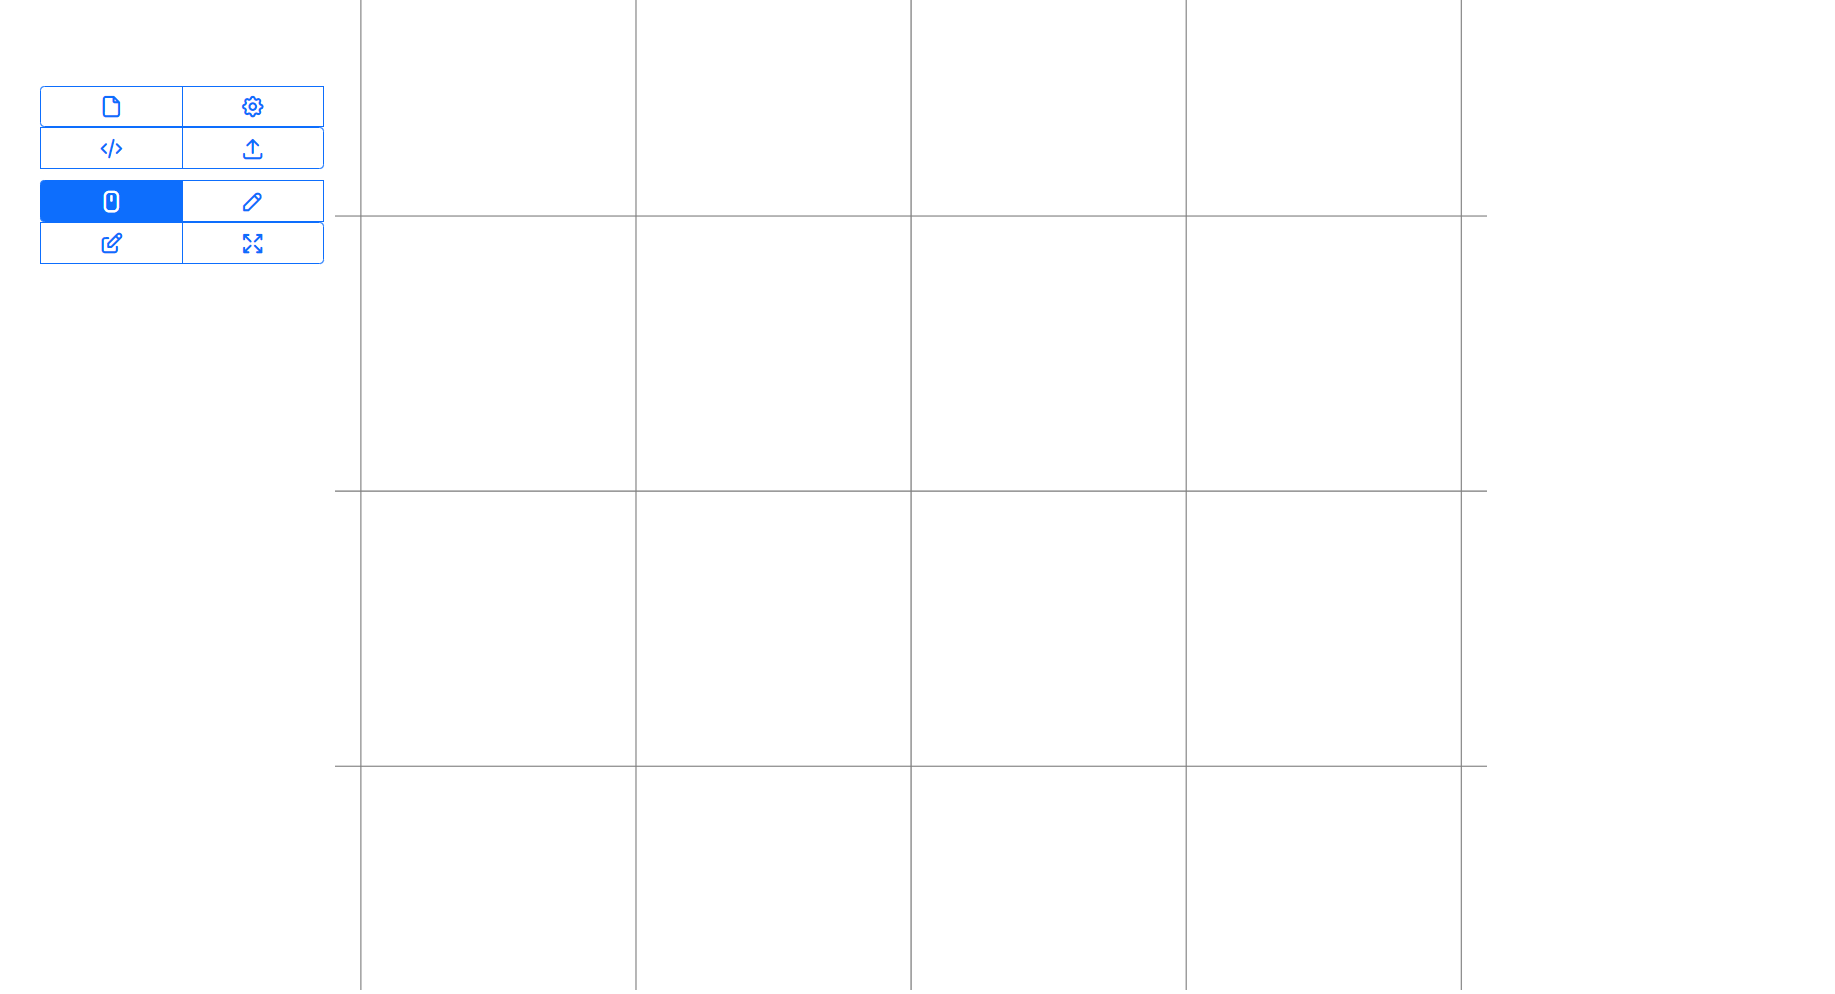
\includegraphics[width=\textwidth]{images/editor_canvas.png}
	\caption{Az elkészült alkalmazás kezdőképernyője}
	\label{fig:canvas}
\end{figure}

Az alkalmazás bármely menüpont alatt támogatja a visszavonás műveleteit: az adott művelet visszavonható a \textit{CTRL + Z} billentyűkombinációval, míg a \textit{CTRL + Y} kombináció lehetőséget biztosít a visszavont művelet megismétlésére. 

\SubSubSection{Vezérlőgombok}

A bal oldalt megjelenő gombok közül a felső mátrix biztosítja az új dokumentum létrehozását, a beállításokat, a meglévő ábra mentését, és visszatöltését.

Az első ikonra 
(
\includegraphics[height=\fontcharht\font`\B]{images/new.png})
kattintva új dokumentumot hozhatunk létre. Ekkor a már meglévő ábra eltűnik, visszatöltésre nincs lehetőség. (\ref{fig:new}. ábra)

\begin{figure}[!h]
	\centering
	
\includegraphics[width=0.85\textwidth]{images/new_modal.png}
	\caption{Új dokumentum létrehozásakor megjelenő figyelmeztető üzenet}
	\label{fig:new}
\end{figure}

A fogaskerék ikonnal 
(
\includegraphics[height=\fontcharht\font`\B]{images/settings.png})
megnyithatjuk a beállításokat, itt van lehetőség az alapértelmezetten bekapcsolt rácsponthoz illeszkedést kikapcsolni, és az előnézetet bekapcsolni.

A következő két ikon felelős a már kész ábra kimentésére 
(
\includegraphics[height=\fontcharht\font`\B]{images/save.png}),
valamint a letöltött ábra visszamásolására
(
\includegraphics[height=\fontcharht\font`\B]{images/load.png}).

Az ábra kimentésekor egy felugró ablak fogad. Ekkor mentésre kerül a jelenlegi vászon állapota is süti formájában. A hivatkozási kód és a \textit{Tikz} kód kimásolható a mezőből gombnyomásra is, valamint egybefűzve le is tölthetők. Ebben az esetben a letöltött \textit{.tex} fájlban egymás alatt jelenik meg a hivatkozási kód, a \textit{TikZ} ábra kódja, valamint a letöltött állomány létrehozásának időpontja. Ezek a \textit{.tex} fájlok módosítás nélkül importálhatók az \lstinline[style=latex]{\input} paranccsal a meglévő dokumentumokba. (\ref{fig:save}. ábra)

\begin{figure}[!h]
	\centering
	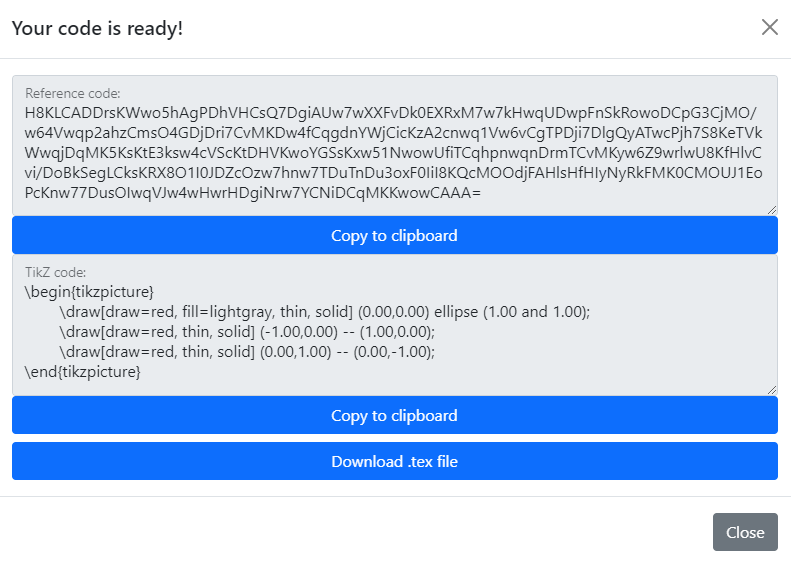
\includegraphics[width=0.85\textwidth]{images/save_modal.png}
	\caption{Az ábra mentésekor megjelenő ablak}
	\label{fig:save}
\end{figure}

Az ábra betöltésekor a már meglévő hivatkozási kód bemásolása után az alkalmazás betölti a kódhoz tartozó ábrát és kezdhetjük is a már meglévő ábra szerkesztését és kibővítését. (\ref{fig:load}. ábra)

\begin{figure}[!h]
	\centering
	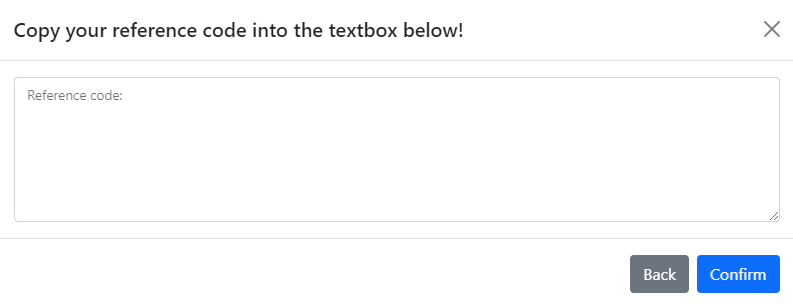
\includegraphics[width=0.75\textwidth]{images/load_modal.png}
	\caption{Az ábra betöltésekor megjelenő ablak}
	\label{fig:load}
\end{figure}

\SubSection{Rajzolás}

A rajzolás mód kiválasztásával megjelennek a vezérlőelemek alatt az alapelemek mátrix alapú felsorolásban és a kijelölt elemhez tartozó tulajdonságok.  (\ref{fig:draw}. ábra)

A megfelelő tulajdonságok beállítása után a rajzolás az egérrel történik. A pont, szöveg és matematikai kifejezések kirajzolása kattintásra történnek, míg a maradék alapelem "drag and drop" (\textit{fogd és vidd}) megoldással kerül kirajzolásra, vagyis a kezdőpont a kattintás helye, és a végpont az egér gombjának felengedésének a pozíciója lesz.

\begin{figure}[!h]
	\centering
	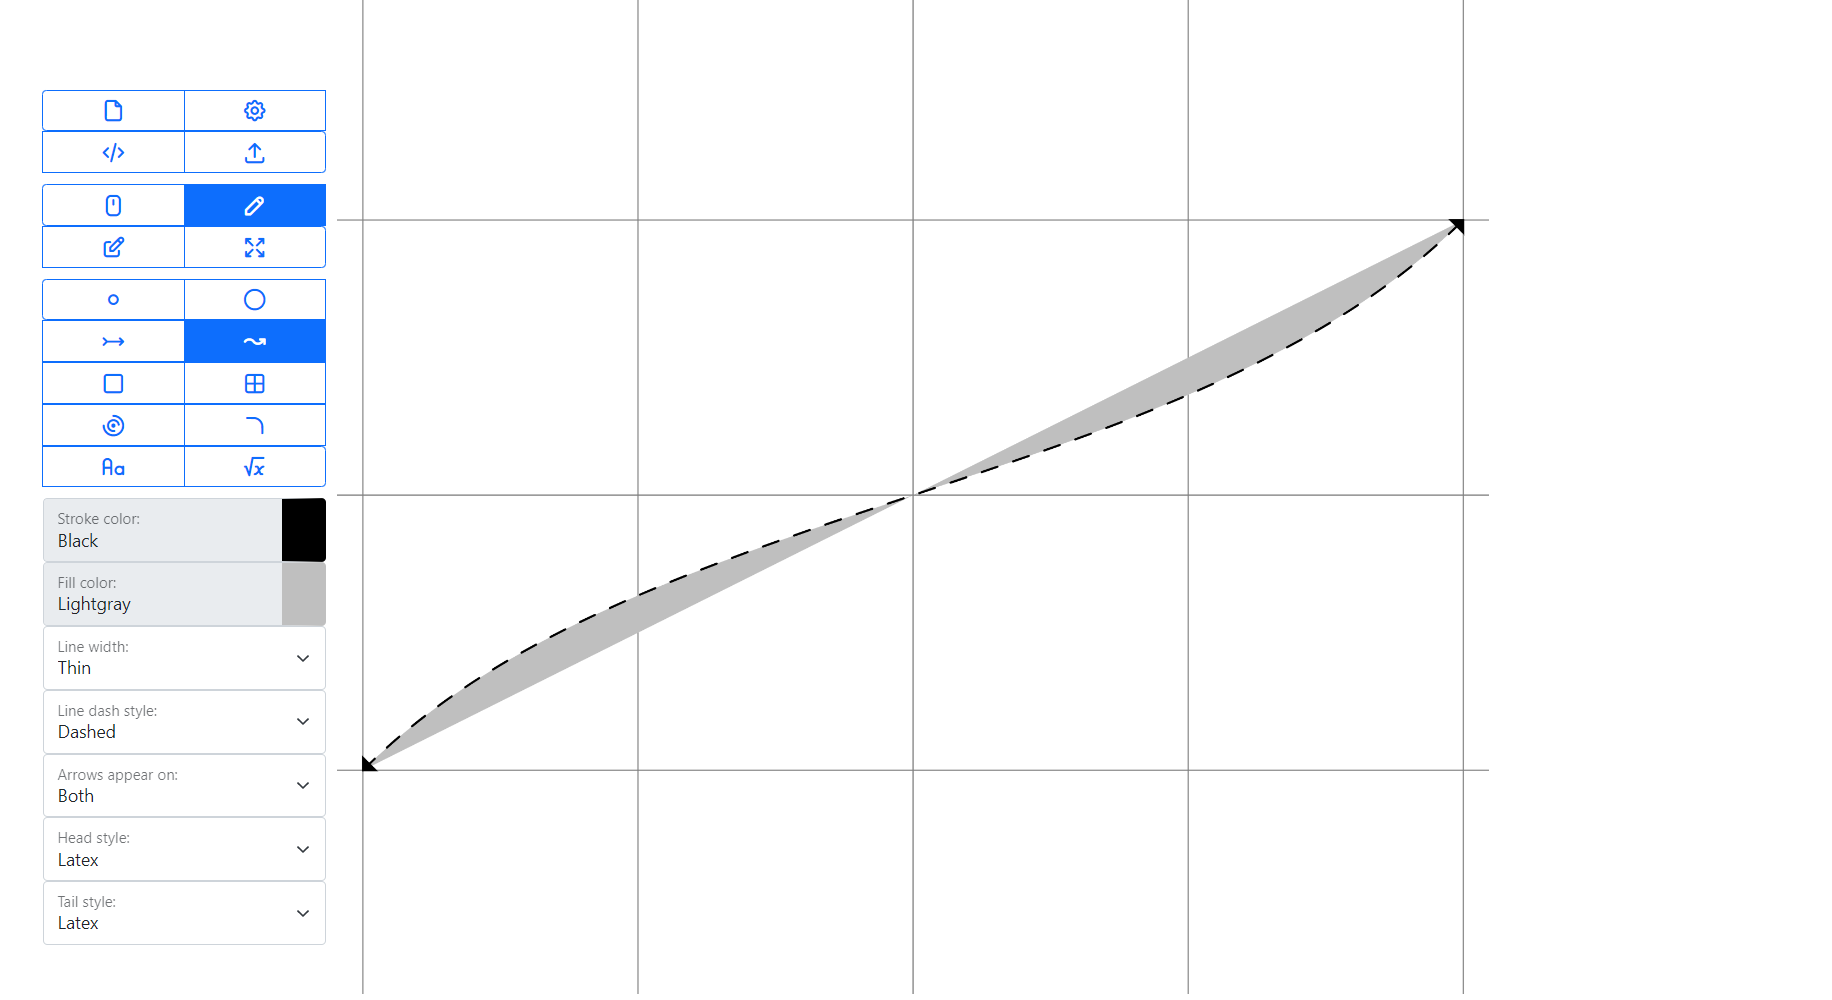
\includegraphics[width=\textwidth]{images/editor_draw.png}
	\caption{A rajzolás funkciói rajzolt elemmel a vásznon}
	\label{fig:draw}
\end{figure}

Amennyiben az előnézet be van kapcsolva a beállításokban, úgy megjelenik az egér helyén egy körvonal, amely jelzi a rajzolandó elem kezdőpontját, valamint a szöveg és a matematikai kifejezések esetében a teljes tartalom megjelenik a beállított tulajdonságok szerint.


\SubSubSection{Matematikai kifejezések elhelyezése}

\begin{figure}[!h]
	\centering
	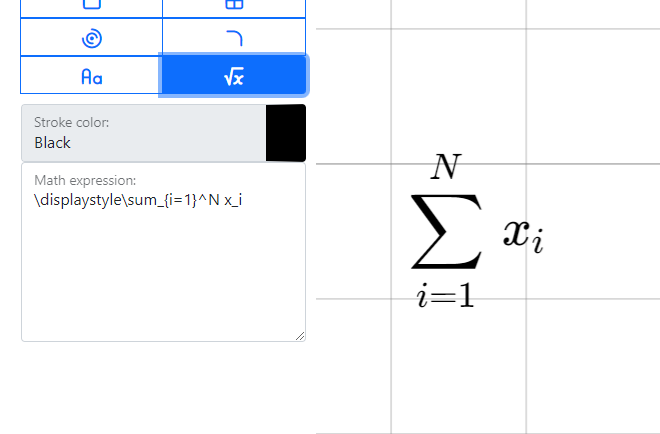
\includegraphics[width=0.5\textwidth]{images/math.png}
	\caption{Példa egy matematikai kifejezés megjelenítésére}
	\label{fig:math}
\end{figure}

A matematikai kifejezések megjelenítéséhez egy szövegdobozba kell megadni a kifejezéseket. A szerkesztő támogatja az egyszerűbb matematikai környezeteket is. (\ref{fig:math}. ábra)


\SubSection{Szerkesztés}

A szerkesztés funkcióban lehetőség van a már lent lévő elemek kiválasztására. A kijelölés téglalap alakú, és a kezdő- és végpont szintén "drag and drop" módszerrel kerül megállapításra. A kijelölés közben egy világosszürke téglalap jelzi az aktuális kijelölt területet, így látszódik mely alapelemek esnek bele. (\ref{fig:edit}. ábra)

\begin{figure}[!h]
	\centering
	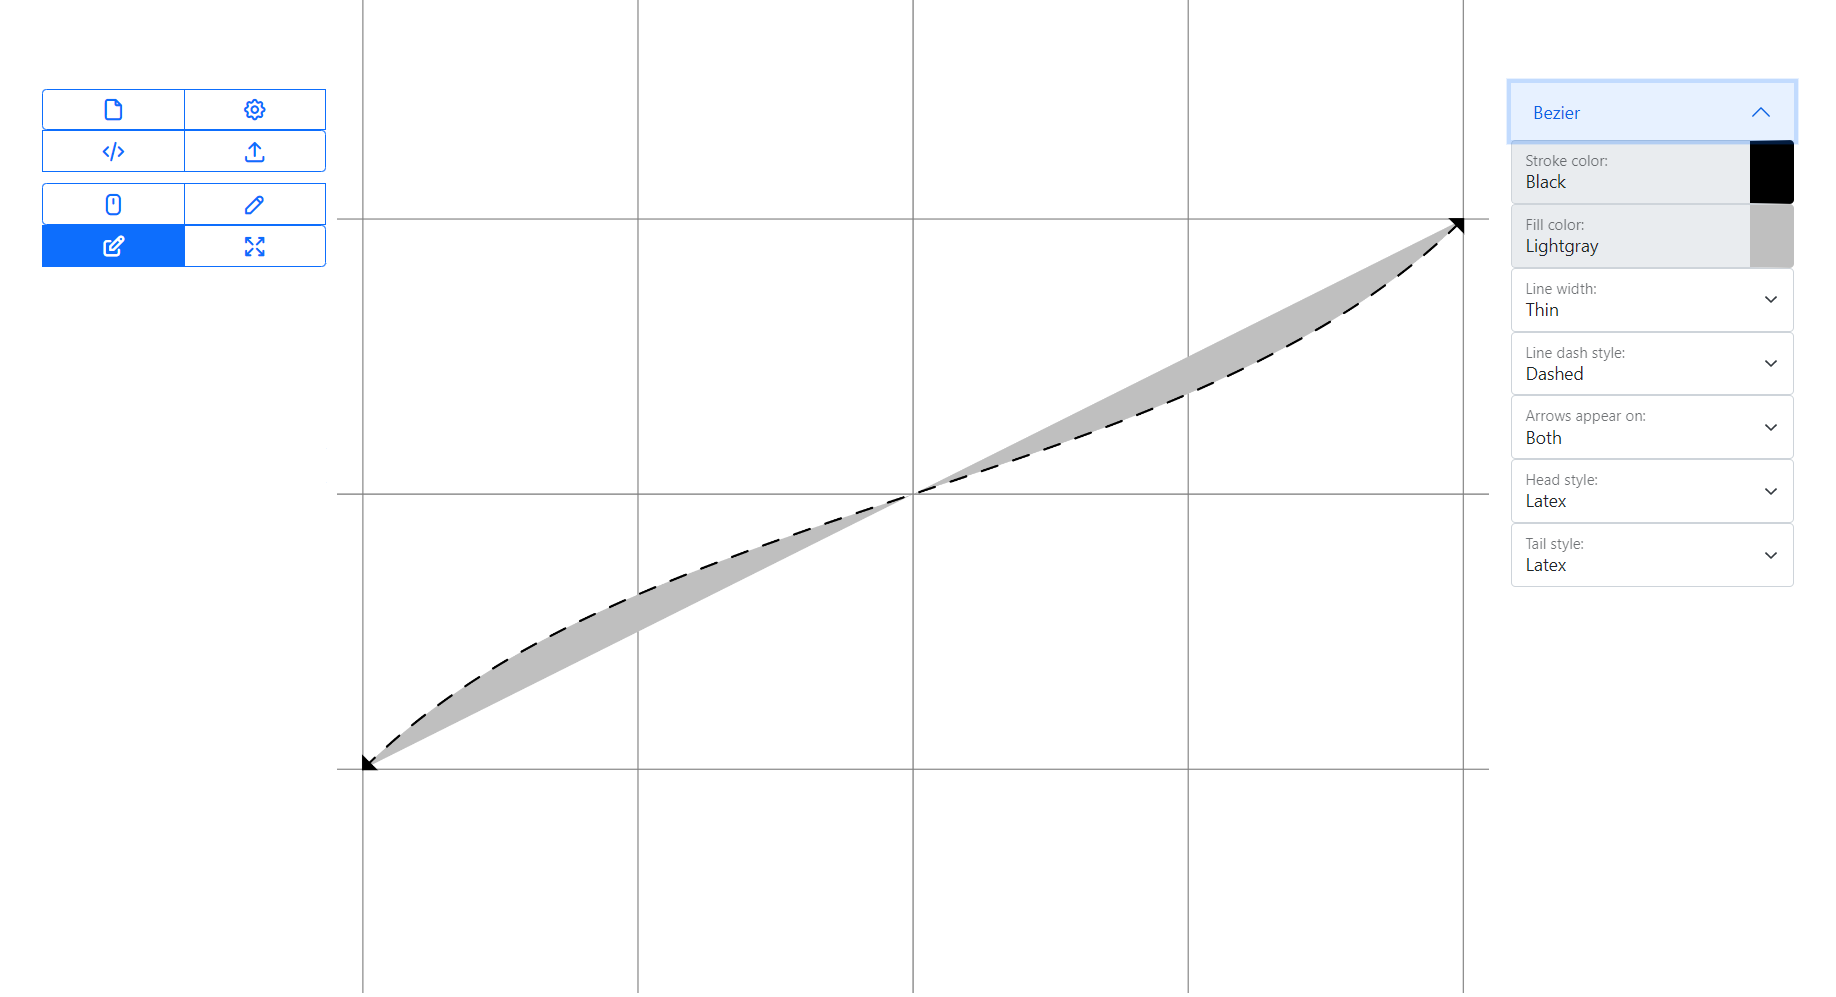
\includegraphics[width=\textwidth]{images/editor_edit.png}
	\caption{A szerkesztés képernyő kiválasztott elem után}
	\label{fig:edit}
\end{figure}

A kijelölés véglegesítése után a rajzoló felület jobb oldalán megjelennek a kijelölt területbe beleeső alapelemek. Itt lehetőség van egyenként szerkeszteni a már lent lévő elemek tulajdonságait. A jelenlegi tulajdonságok automatikusan betöltődnek, módosításkor a vásznon automatikusan megjelenik, nincs szükség a módosítás mentésére.

Kijelölés után lehetőségünk van a másolásra, beillesztésre és törlésre egyaránt, ezek mindegyike billentyű lenyomásra működnek. A másolás a  \textit{CTRL + C}, a beillesztés a \textit{CTRL + V}, még a törlés a \textit{CTRL + X} billentyűkombinációval, és a \textit{DELETE} billentyűvel egyaránt működik.

\SubSection{Mozgatás}

A mozgatás funkcióban lehet a már lent lévő ábrák pontjait kijelölés után mozgatni. A mozgatandó elem kijelölése kattintásra történik, \textit{CTRL} billentyű lenyomása közben van lehetőség több pont kijelölésére. A mozgatás szintén "drag and drop" megoldással működik. A kijelölt pont a kezdeti zöld helyett piros színre vált, és egér gombbal mozgatható. A felengedéssel egy időben, ha be van kapcsolva a rácspontra mozgatás, akkor ebben az esetben is megtörténik.  (\ref{fig:move}. ábra)

\begin{figure}[!h]
	\centering
	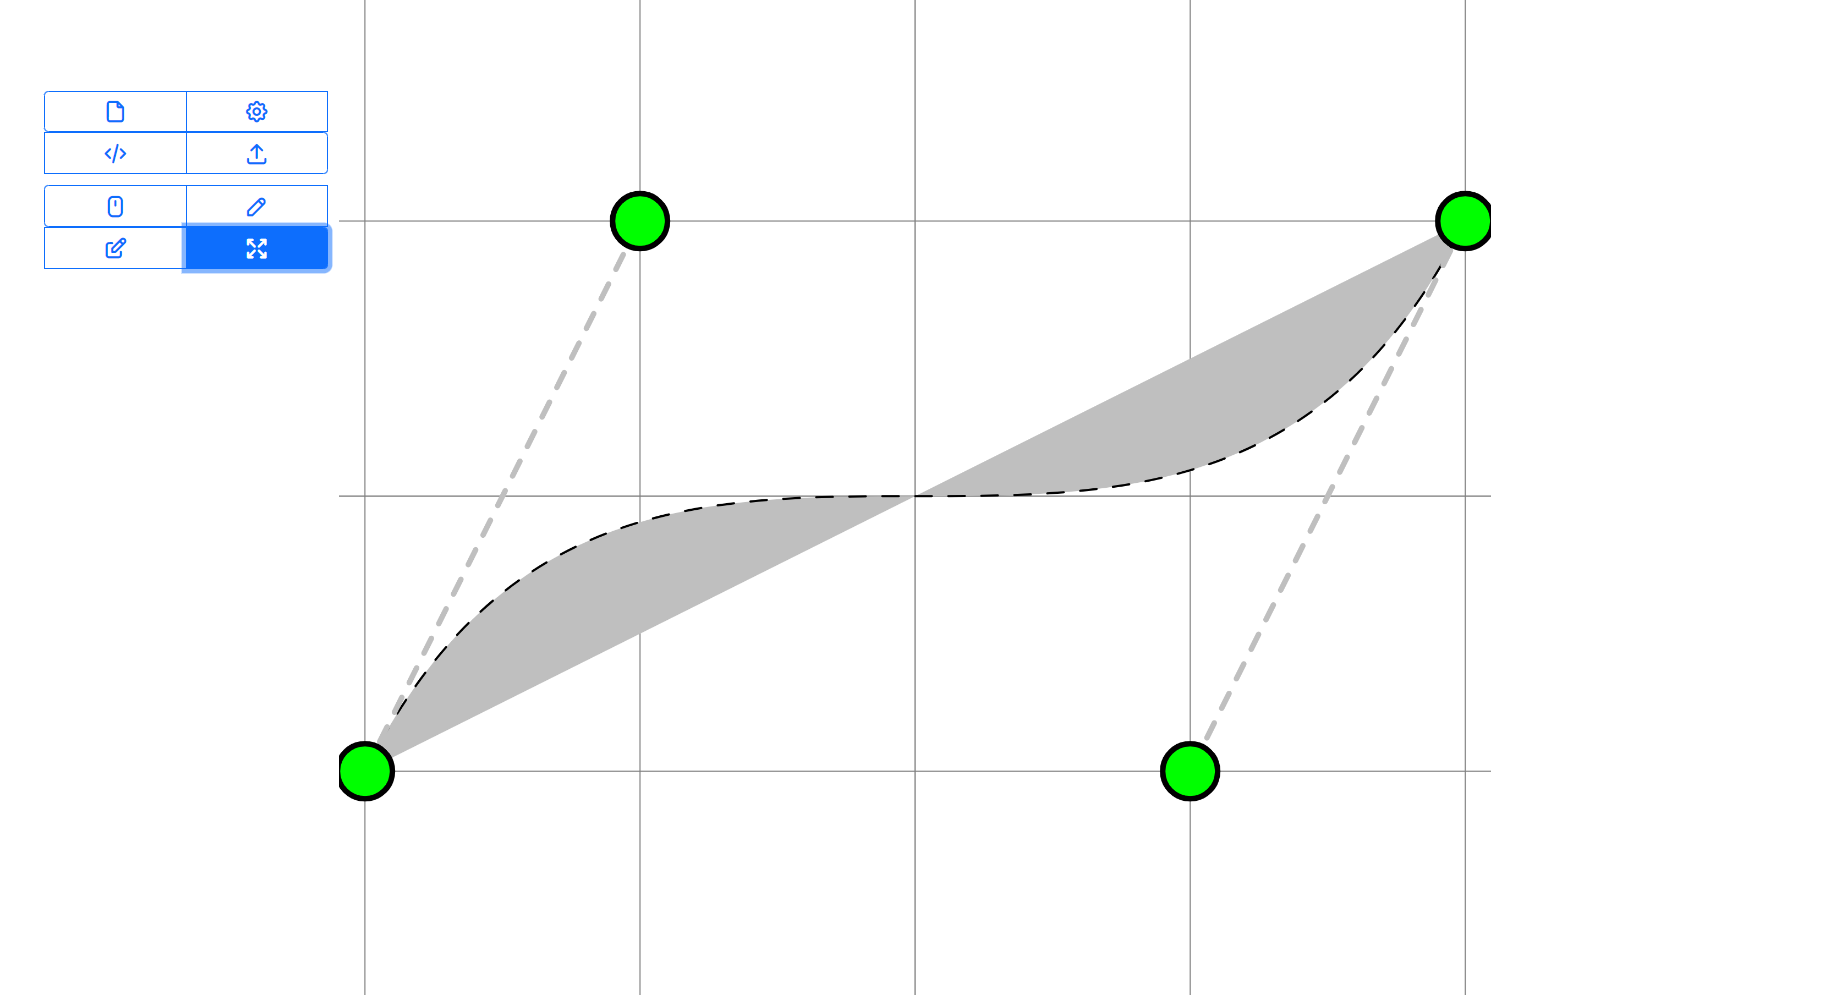
\includegraphics[width=\textwidth]{images/editor_move.png}
	\caption{A mozgatásra alkalmas pontok megjelenítése a vásznon}
	\label{fig:move}
\end{figure}

\Section{Definiált osztályok bemutatása}

A definiált osztályok UML diagramját a \ref{fig:uml}. ábra tartalmazza, és ezek kerülnek részletezésre a következő szakaszokban.

\begin{figure}[!h]
	\centering
	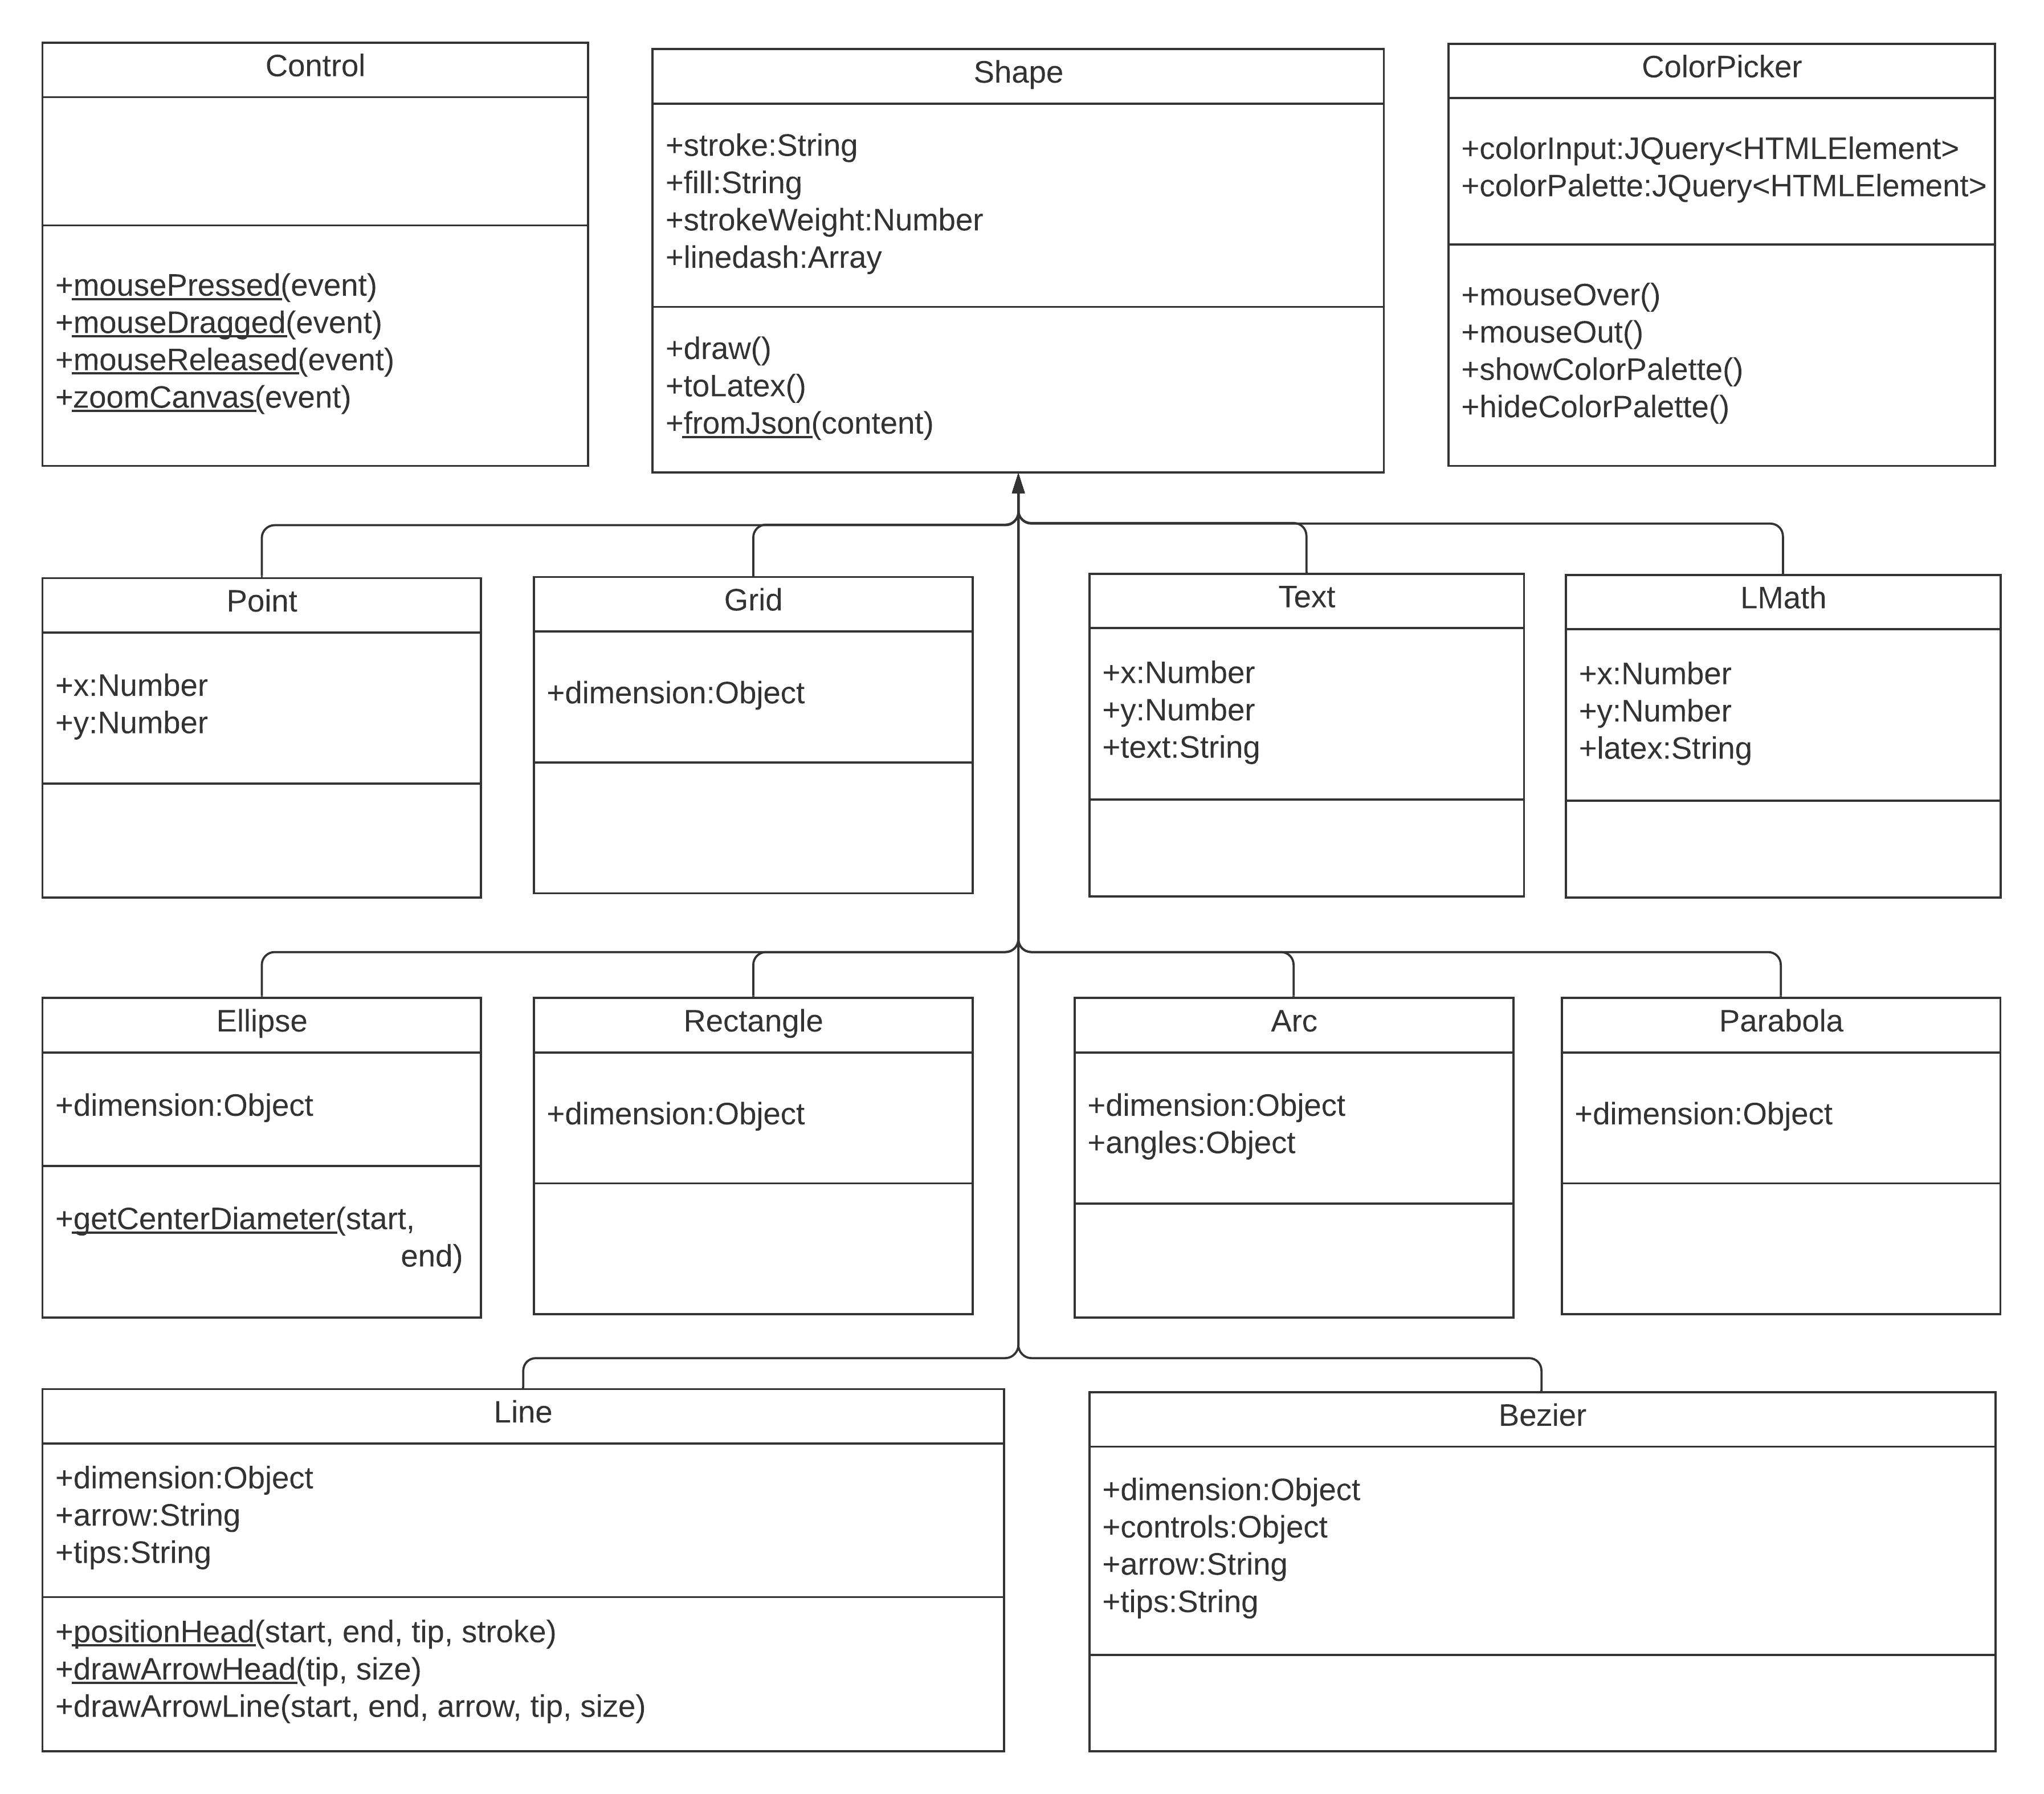
\includegraphics[width=\textwidth]{images/uml.png}
	\caption{Az osztályok UML diagrammja}
	\label{fig:uml}
\end{figure}

\SubSection{Alapelemek osztályai}

Ebbe a részbe kerülnek a menüben kiválasztható alapelemek osztályai, valamint az aktuális elem esetében a  \textit{p5.js} és \textit{TikZ} közötti különbségek és megoldásuk. 

\SubSubSection{Shape osztály}

A \textit{Shape} osztály minden alapelem szülője, itt kerül beállításra majdnem az összes elemnél előforduló szín, betűszín, vonal vastagság és mintázat. A \textit{draw} metódus beállítja a megadott tulajdonságokat a rajzolás előtt. A \textit{toLatex} és a \textit{fromJson} metódusok még itt üresek, értékeket a származtatott osztályokban kapnak.

\SubSubSection{Point osztály}

A \textit{Point} osztály egy pont tulajdonságait tárolja. Példányosítás során meg kell adni a pont két koordinátáját, és a tulajdonságokat tömb formájában. A jobb láthatóság érdekében \textit{p5.js} és \textit{TikZ} esetében egy kis méretű kör kerül kirajzolásra. 

\SubSubSection{Ellipse osztály}

Az \textit{Ellipse} osztály ellipszis rajzolását teszi lehetővé. A példányosításhoz meg kell adni két koordinátapárt (egy x és egy y koordinátát), valamint a tulajdonságokat. 

A \textit{p5.js} és a \textit{TikZ} is ugyanúgy támogatja az ellipszis rajzolását: meg kell adni a középpontot és a sugár méretét, így szükséges egy metódus, ami ezt kiszámolja. A \textit{getCenterDiameter} metódus ezt teszi lehetővé:

\begin{lstlisting}[style=es6]
static getCenterDiameter(start, end) {
	let center = {
		x: start.x + (end.x - start.x) / 2,
		y: start.y + (end.y - start.y) / 2
	};

	let diameter = {
		x: end.x - start.x,
		y: end.y - start.y
	};
	return {center, diameter}
}
\end{lstlisting}

\SubSubSection{Line osztály}

A \textit{Line} osztályban vannak definiálva a vonal rajzolásához szükséges metódusok. A példányosításhoz meg kell adni két koordinátapárt (egy x és egy y koordinátát), valamint a tulajdonságokat. A nyilak rajzolását is ez az osztály végzi, ugyanis tulajdonságként megkapja, hogy hol és milyen típusú nyíl kirajzolása szükséges. 

A \textit{p5.js} megvalósítás kicsit komplikáltabb, mint a \textit{TikZ} megoldás. A \textit{p5.js} esetében a \textit{positionHead} metódus a kiválasztott végpontra lép, a \textit{drawArrowHead} metódus pedig az aktuális pontra kirajzolja a kiválasztott nyílhegyet. A \textit{drawArrowLine} metódus csak egyszerűen összeköti a két végpontot a nyílhegy függvényében. A \textit{TikZ} esetében pedig csak a \textit{draw} paramétereként meg kell adni a nyílhegyet.

\SubSubSection{Bezier osztály}

A \textit{Bezier} osztály egy harmadfokú Bézier-görbe kirajzolását teszi lehetővé. A példányosításhoz meg kell adni két koordinátapárt (egy x és egy y koordinátát), valamint a tulajdonságokat. A program automatikusan számol lerakáskor két kontrollpontot a harmadolópontok helyére, mely utólag természetesen módosítható. A vonalaknál látott nyílhegyek itt is elérhetők.

A \textit{p5.js} és a \textit{TikZ} megadás rendre megegyezik: először meg kell adni a kezdőpontot, majd a két kontrollpontot és végül a végpontot.

\SubSubSection{Rectangle osztály}

A \textit{Rectangle} osztály egy tetszőleges téglalap létrehozására szolgál. A példányosításhoz meg kell adni két koordinátapárt (egy x és egy y koordinátát), valamint a tulajdonságokat. 

A \textit{p5.js} és a \textit{TikZ} megadás megegyezik: meg kell adni a kezdő- és a végpontot, amennyiben a \textit{p5.js} esetében megadjuk előtte, hogy a pontok a szemközti sarkakat jelölik a kezdőpont, a magasság és szélesség helyett. Erre szolgál a \textit{rectMode(CORNERS);} metódus és paramétere.

\SubSubSection{Grid osztály}

A \textit{Grid} osztály egy rácsháló létrehozását teszi lehetővé.  A példányosításhoz meg kell adni két koordinátapárt (egy x és egy y koordinátát), valamint a tulajdonságokat. 

A \textit{p5.js} nem rendelkezik rácsháló kirajzolásához beépített függvénnyel, így saját megoldással történik a kirajzolás: a kezdőpont és a végpont között függőlegesen és vízszintesen is vonalak kerülnek kirajzolásra így megkapva a hálót.

A \textit{TikZ} alapból rendelkezik ezzel a funkcióval, ebben az esetben csak a két pont megadása szükséges.

A rácsháló kirajzolását végző kódrészlet:

\begin{lstlisting}[style=es6, morekeywords={P5}]
for (let i = Math.min(this.dimension.start.x, this.dimension.end.x); 
     i <= Math.max(this.dimension.start.x, this.dimension.end.x); 
     i += grid_density) {
         P5.line(i, this.dimension.start.y, i, this.dimension.end.y)
}

for (let i = Math.min(this.dimension.start.y, this.dimension.end.y); 
    i <= Math.max(this.dimension.start.y, this.dimension.end.y); 
    i += grid_density) {
        P5.line(this.dimension.start.x, i, this.dimension.end.x, i)
}
\end{lstlisting}

\SubSubSection{Arc osztály}

Az \textit{Arc} osztály egy körív rajzolását teszi lehetővé. A példányosításhoz meg kell adni két koordinátapárt (egy x és egy y koordinátát), valamint a tulajdonságokat. A tulajdonságok között szerepel az ív kezdő és végpontja fokban az adott sugarú körön.

A kezdőpont és a sugár meghatározásához itt is a \textit{Ellipse} osztálynál megismert \textit{getCenterDiameter} metódus szolgál. 

A \textit{p5.js} és a \textit{TikZ} egyaránt rendelkezik beépített megoldással körív rajzolására, azonban máshogy kerülnek kirajzolásra. A \textit{p5.js} esetében a középpont és az azon lévő köríven a megadott fokok, míg a \textit{Tikz} esetében a megadott pont a kezdőpont, és onnan kerül a körív kirajzolásra, nem a középpont a mérvadó. Az exportált \textit{TikZ} a \textit{p5.js} megoldásával egyezik meg, vagyis a kezdőpontba el van tolva a megfelelő irányba.

\SubSubSection{Parabola osztály}

A \textit{Parabola} osztályban vannak definiálva egy parabola kirajzolásához szükséges metódusok. A példányosításhoz meg kell adni két koordinátapárt (egy x és egy y koordinátát), valamint a tulajdonságokat.

A \textit{p5.js} nem rendelkezik parabola kirajzolásához beépített függvénnyel, így saját megoldással történik a \textit{TikZ}-ben szereplő parabola kirajzolása. 

A \textit{TikZ} parabola egyenlete: 

$$\displaystyle y = \frac{y_1 - y_0}{(x_1 - x_0)^2}(x - x_0)^2 + y_0, \qquad x\in[x_0, y_0].$$

\noindent
A kódrészlet, amely a vászonra rajzolja ennek az egyenletnek a képét:

\begin{lstlisting}[style=es6, morekeywords={P5}]
let a = (this.dimension.end.y - this.dimension.start.y) / 
    Math.pow(this.dimension.end.x - this.dimension.start.x, 2);
if (isFinite(a)) {
	P5.beginShape();
	for (let i = Math.min(this.dimension.start.x, this.dimension.end.x); 
	    i <= Math.max(this.dimension.start.x, this.dimension.end.x); 
	    i += 0.25) {
		    P5.vertex(i, a * (Math.pow(i - this.dimension.start.x, 2)) +
		        this.dimension.start.y)
	}
	P5.endShape();
} else {
	P5.line(this.dimension.start.x, this.dimension.start.y, 
	    this.dimension.end.x, this.dimension.end.y)
}
\end{lstlisting}

\SubSubSection{LMath osztály}

A \textit{LMath} osztály matematikai kifejezések létrehozását teszi lehetővé. Példányosítás során meg kell adni a pont két koordinátáját, és a tulajdonságokat, mely között szerepel a kirajzolandó kifejezés. 

A \textit{p5.js} nem támogatja a \LaTeX\ kifejezések megjelenítését a vásznon, így egy másik függvénykönyvtár használatával kellett megoldani: ez pedig a KaTeX \cite{katex}, mely egy gyors, könnyen használható JavaScript könyvtár a \LaTeX\ matematikai kifejezések webes megjelenítéséhez.

A \textit{renderToCanvas} függvénnyel lehet a KaTeX által generált kifejezéseket a vászonra rakni, paraméterként meg kell adni a kirajzolandó kifejezést, magát a vásznat, mint kirajzolási hely, valamint a kifejezés pozícióját (az x és y koordinátát egyaránt).

\begin{lstlisting}[style=es6, morekeywords={document, P5, katex}]
let canvas = document.getElementById(P5.canvas.id);
katex.renderToCanvas(this.latex, canvas, 
    this.x + grid_density / 8, this.y - grid_density / 2.5, 
        { fontSize: 19.5 }
);
\end{lstlisting}

A \textit{TikZ} megoldás egyszerűbb, ott egy \textbackslash \textit{node} parancs paramétereként kell megadni a kifejezést matematikai módban.

\SubSubSection{Text osztály}

A \textit{Text} osztály szöveg vászonra helyezését teszi levetővé. A példányosítás ugyanúgy zajlik, mint a matematikai kifejezések esetében.

Annak ellenére, hogy a \textit{p5.js} rendelkezik olyan funkciókkal ezek "kirajzolása" szintén a KaTeX függvénykönyvtár segítségével történik, annyi eltéréssel, hogy a kirajzolandó szöveg megkapja a \textbackslash text\{\} paramétert, hogy ne érvényesüljön a matematikai mód.

\begin{lstlisting}[style=es6, morekeywords={document, P5, katex}]
let canvas = document.getElementById(P5.canvas.id);
katex.renderToCanvas(`\\text{${this.text}}`, canvas, 
    this.x + grid_density / 8, this.y - grid_density / 2.5,
    { fontSize: 19.5 }
);
\end{lstlisting}

A \textit{TikZ} megoldás hasonlóan matematikai kifejezésekhez, a \textbackslash \textit{node} parancs paramétereként kell megadni a szöveget.

\SubSection{Funkciók osztályai}

Itt a két funkció kerül bemutatásra, ami osztályba lett szedve a könnyebb elérés miatt. A funkciók jelentős része modulként szerepel az alkalmazásban, nem osztályokba csoportosítva.

\SubSubSection{Control osztály}

Ez az osztály felelős a vászon mozgatásáért és a nagyításért. Az osztályban eseménykezelők kerültek létrehozásra: kezelésre kerül az egér kattintása, húzása, felengedése valamint a görgetés. A vászon mozgatása szintén a "drag and drop" elvet követi.

Az eseménykezelők beállítása a \textit{p5.js} példányára, amely a \textit{sketch}-ben kerül létrehozásra:

\begin{lstlisting}[style=es6, morekeywords={P5, Control}]
P5.mousePressed = e => Control.mousePressed(e)
P5.mouseDragged = e => Control.mouseDragged(e);
P5.mouseReleased = e => Control.mouseReleased(e);
P5.mouseWheel = e => Control.zoomCanvas(e);
\end{lstlisting}

\SubSubSection{ColorPicker osztály}

Ez az osztály kezeli az alkalmazásban szereplő színválasztó megfelelő működését. Itt kerül kezelésre az adott színválasztó kiválasztása, a színpaletta megjelenítésé és eltüntetésé, az adott szín kijelölése.   (\ref{fig:cp2}. ábra)

\begin{figure}[!h]
	\centering
	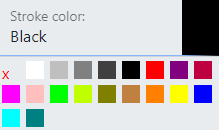
\includegraphics[width=0.3\textwidth]{images/colorpicker.png}
	\caption{Példa a színek kiválasztására}
	\label{fig:cp2}
\end{figure}

A színválasztó előredefiniált színek alapján dolgozik, ezek megegyeznek a \LaTeX\ által definiáltakkal:

\begin{lstlisting}[style=es6]
const COLOR = {
	NONE: "#E9ECEF", // for no stroke or fill color
	WHITE: "#FFFFFF",
	LIGHTGRAY: "#BFBFBF",
	GRAY: "#808080",
	DARKGRAY: "#404040",
	BLACK: "#000000",
	RED: "#FF0000",
	VIOLET: "#800080",
	PURPLE: "#BF0040",
	MAGENTA: "#FF00FF",
	PINK: "#FFBFBF",
	GREEN: "#00FF00",
	LIME: "#BFFF00",
	OLIVE: "#808000",
	BROWN: "#BF8040",
	ORANGE: "#FF8000",
	YELLOW: "#FFFF00",
	BLUE: "#0000FF",
	CYAN: "#00FFFF",
	TEAL: "#008080"
}
\end{lstlisting}

Azért ilyen formában kerülnek tárolásra a színkódok, mert a \textit{p5.js} tudja kezelni a hexadecimális színkódokat. A \textit{COLOR}-ra hivatkozva meg tudjuk adni a színeket. Például piros körvonal, és világosszürke kitöltés esetében:
\begin{lstlisting}[style=es6, morekeywords={P5, COLOR}]
P5.stroke(COLOR.RED);
P5.fill(COLOR.LIGHTGRAY);
\end{lstlisting}